\chapter{Operation and Installation} \label{ch:Usage}

\section{Operating Principle}

Digifiz Replica dashboards reuse the original Volkswagen enclosure, the factory connectors, and either the mechanical speedometer cable or an electronic speed sensor.
Replica variants employ a fiberglass main PCB populated with discrete components driven by an ATmega~2560 microcontroller and MAX~7219 indicator drivers.
Replica Next builds on an ESP32-S3 system-on-chip and introduces a new SLA-printed enclosure, front panel, and connector adapter, illuminated by WS2812 addressable LEDs.

\section{Technical Specifications}

Both generations operate from the vehicle's 9--16~V electrical system.
Replica Next draws approximately 13~mA from the battery in standby; Replica consumes no standby current when fully powered down.
The shared measurement capabilities are:
\begin{itemize}
    \item \textbf{Vehicle speed:} acquired via the mechanical or electronic speed sensor, with a systematic error of 10~km/h and a relative error of 3~km/h.
          The displayed value saturates at 999~km/h (or mph for imperial configurations).
    \item \textbf{Engine speed:} derived from the ignition signal through an RC-limited optocoupler stage (430~nF/1.2~k\ohm{} with diode clamping).
          The systematic and relative errors are within 200~rpm.
    \item \textbf{Fuel level:} measured with the resistive tank sender; the typical uncertainty is 10~litres.
    \item \textbf{Coolant temperature:} indicated on the scale using the OEM thermistor (quantitative calibration is not provided).
    \item \textbf{Time:} the real-time clock is accurate to within one minute; Replica uses a DS3231 with a CR2032 backup cell, while Replica Next keeps time through firmware.
    \item \textbf{Tell-tale indicators:} direction indicators, high beam, oil pressure warnings, generator status, handbrake, rear window heating or diesel glow-plug, and front/rear fog lights.
\end{itemize}

\section{Operating Conditions and Safety}

\subsection{Environmental Limits}

\begin{itemize}
    \item Operating temperature: \(-40\,^{\circ}\mathrm{C}\) to \(+70\,^{\circ}\mathrm{C}\) with up to 95\% relative humidity.
    \item Year-round operation inside the passenger compartment is supported, even when the vehicle is parked.
    \item Storage is permitted inside the vehicle cabin or indoors between \(+15\,^{\circ}\mathrm{C}\) and \(+40\,^{\circ}\mathrm{C}\); avoid prolonged direct sunlight.
\end{itemize}

\subsection{Responsibilities}

\begin{itemize}
    \item The dashboards are hobbyist-grade devices intended for project cars; they are not certified measuring instruments.
    \item Installations are performed at the owner's risk. If readings are questionable, corroborate them with the vehicle's factory gauges or independent instruments.
    \item Do not integrate Digifiz readings into automated control systems.
    \item Warranty coverage extends for one year when the authors perform the installation and for two weeks when installed independently; malfunctions within these periods will be repaired by the authors.
\end{itemize}

\section{Preparation and Installation}

Follow the sequence below when replacing the factory cluster:
\begin{enumerate}
    \item Remove the plastic trim covering the pedals and dashboard to expose the instrument cluster.
    \item Disconnect the vehicle battery.
    \item Unplug the factory harness from the instrument panel.
    \item Disconnect the mechanical speedometer cable (if present).
    \item Unscrew the cluster from its brackets and carefully remove it.
    \item Route the temperature and speed sensor harnesses supplied with the Digifiz kit.
    \item Install the new dashboard into the bracket grooves and secure it with screws.
    \item For Replica Next, connect the VW MFA sensors or compatible replacements and route the cables to the CE~1/CE~2 connectors.
    \item On single-connector variants (\texttt{GACS}/\texttt{GARS}/\texttt{DARS}/\texttt{DACS}), connect the labelled MFA\_MODE, MFA\_RESET, MFA\_BLOCK, and handbrake wires manually if the vehicle harness lacks these contacts.
    \item Plug in the harness(es) and connect the electronic speed sensor or speedometer cable as required.
    \item Reinstall the dashboard trim and pedal cover in the reverse order.
\end{enumerate}

\section{Daily Operation and MFA Features}

\subsection{Startup Behaviour}

The dashboard powers up automatically with ignition.
When energised, the cluster performs a self-test, illuminating the speed scale before stabilising at the current RPM.
Lighting follows the vehicle sidelights, and the MFA controller begins collecting data once the vehicle is in motion.

\subsection{MFA Functions}

Six MFA pages are available:
\begin{enumerate}
    \item Daily operating time.
    \item Trip distance.
    \item Fuel consumption (not implemented on the first Replica revision).
    \item Average speed (displayed as the value multiplied by ten).
    \item Engine oil temperature (external harness required).
    \item Ambient temperature (external harness required).
\end{enumerate}

On Replica dashboards a capacitive touch point behind the VW badge controls the MFA.
Replica Next requires an external steering column switch.
Touch durations behave as follows:
\begin{itemize}
    \item Short press (\(<1\)~s): cycle to the next MFA function.
    \item Medium press (1--3~s, when no steering column switch is present): switch between MFA memory blocks.
    \item Long press (3--7~s): reset the active MFA function (affects consumption, trip distance, elapsed time, and average speed).
\end{itemize}

\subsection{Backlight Control}

Replica dashboards provide a small manual brightness trim above the parking-light switch, while Replica Next relies on automatic brightness via an onboard photodiode.
Automatic control can be overridden through configuration commands (\Cref{ch:Features}).

\subsection{Indicator Layout}

The layout of the horizontal indicator block and the on-screen labelling are shown in \Cref{fig:indicator-layout,fig:indicator-legend}.

\begin{figure}[htbp]
    \centering
    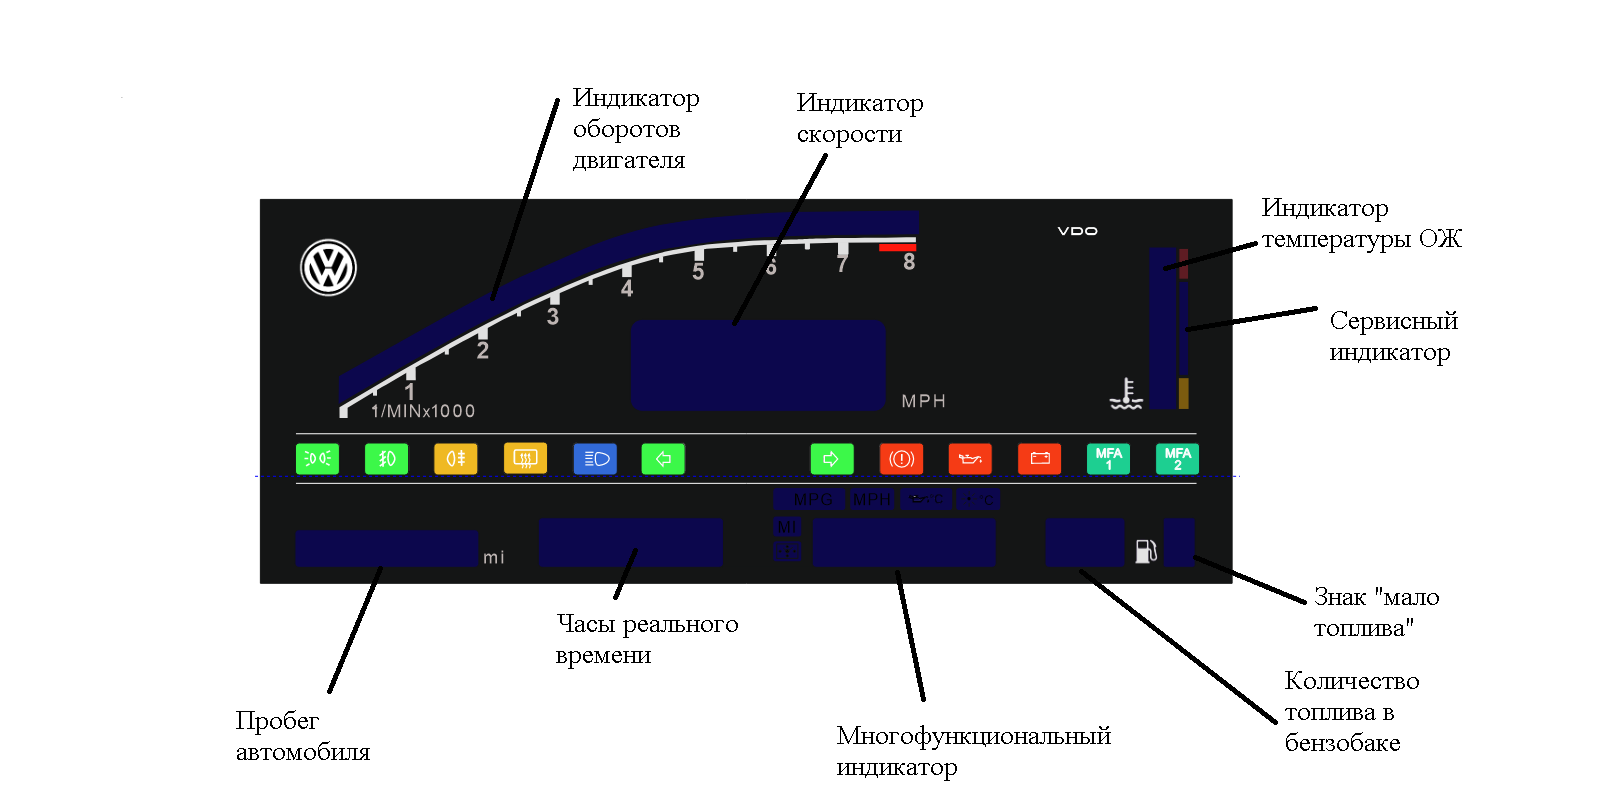
\includegraphics[width=0.85\textwidth]{digifiz_manual/image017.png}
    \caption{Indicator layout displayed during the power-on self-test.}
    \label{fig:indicator-layout}
\end{figure}

\begin{figure}[htbp]
    \centering
    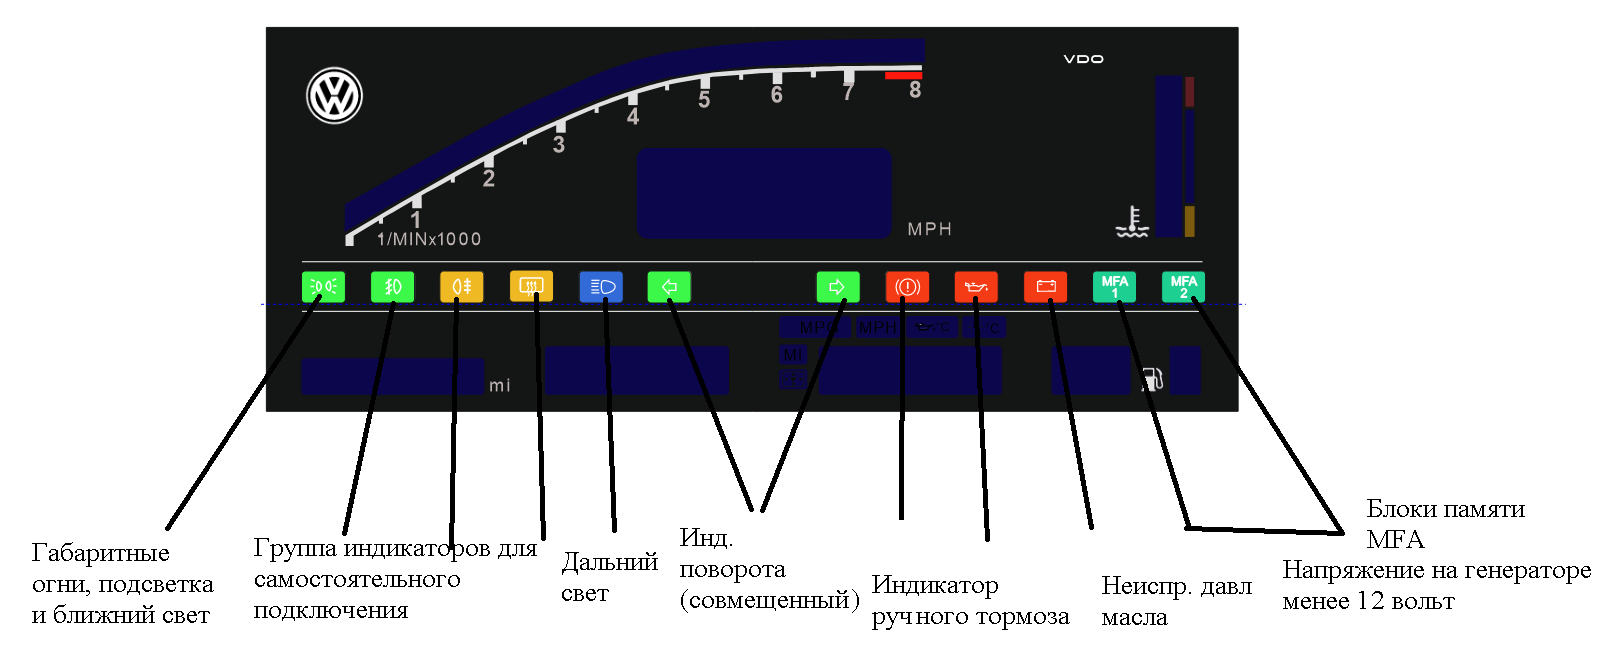
\includegraphics[width=0.8\textwidth]{digifiz_manual/image018.png}
    \caption{Legend for the horizontal indicator group.}
    \label{fig:indicator-legend}
\end{figure}

\subsection{Maintenance Interfaces}

Replica dashboards expose configuration interfaces for both generations:
\begin{itemize}
    \item Classic Digifiz Replica units include a Bluetooth 2.0 (or BLE-compatible) module.
          Install the \emph{Serial Bluetooth Terminal} application from Google Play, pair with the dashboard, and issue commands directly from the terminal view.
          Apple iOS devices cannot connect to the module.
    \item Replica Next exposes an embedded Wi-Fi access point that provides the configuration portal documented in \Cref{ch:Features}.
          Disable mobile data while connecting to ensure the captive portal loads correctly.
\end{itemize}

Both generations also accept configuration commands over the USBasp programming interface when the dashboard is connected to a computer, which powers the unit for bench testing.

\section{Classic Replica Maintenance} \label{sec:classic-maintenance}

Classic Digifiz Replica dashboards require several periodic care steps to remain operational.

\subsection{Front Panel Care}

The plexiglass screen is UV printed and can be marred by sharp objects.
Avoid abrasive cleaners and protect the panel during installation or storage; cosmetic damage is not covered by warranty.

\subsection{Backup Battery}

The integrated DS3231 real-time-clock module uses a replaceable CR2032 cell with an expected life of approximately four years.
When the dashboard begins losing time after each power cycle, remove the rear cover, replace the battery without disconnecting the harness, and dispose of the depleted cell responsibly.

\subsection{USBasp Programming}

Each dashboard ships with a USBasp programmer and a pre-installed wiring harness.
Install the required driver (for example via \url{https://myrobot.ru/downloads/driver-usbasp-v-2.0-usb-isp-windows-7-8-10-xp.php}) before connecting the programmer to a Windows host.
Connecting the programmer powers the dashboard, allowing firmware updates and diagnostic checks without the vehicle.

\begin{figure}[htbp]
    \centering
    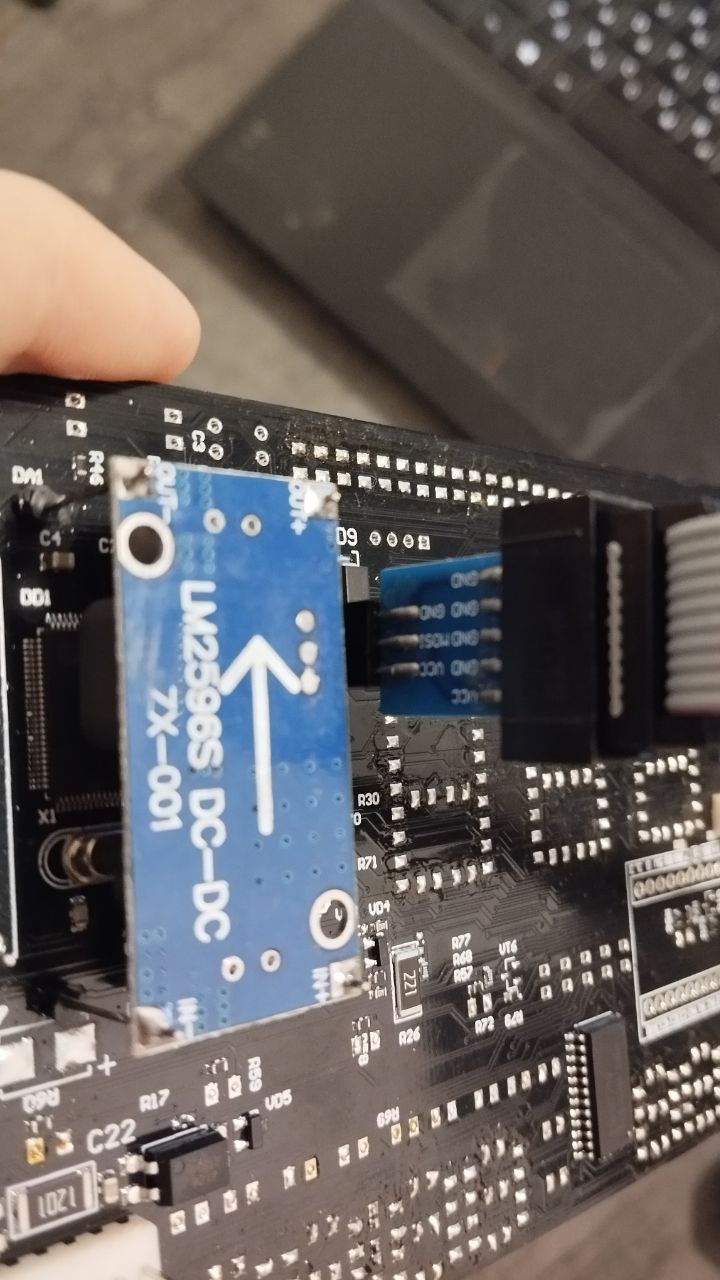
\includegraphics[width=0.35\textwidth]{digifiz_manual/image048.png}
    \caption{USBasp programming cable orientation on the classic Replica PCB.}
    \label{fig:usbasp-orientation}
\end{figure}

The recommended \texttt{avrdude} invocation for reflashing an ATmega~2560-based dashboard (wrapped across two lines for readabi
lity) is:
\begin{verbatim}
avrdude -c usbasp -p m2560 -e -U lfuse:w:0xff:m -U hfuse:w:0x99:m
    -U efuse:w:0xff:m -U flash:w:Digifiz.ino.mega.hex
\end{verbatim}

After a successful flash, press the capacitive touch button four or five times to initialise the MFA memory blocks.
If the memory fails to populate, repeat the flashing procedure or issue the Bluetooth command \verb|252 0| to perform a factory reset.

\subsection{Firmware Availability}

Compiled firmware images and source code are maintained at \url{https://github.com/Sgw32/DigifizReplica} (\Cref{ch:Design}).
Keep a record of the odometer value and restore it with command \verb|11 <mileage>| after reflashing when necessary.
